% Put labels, etc., on figures using PSTricks.
% Use dvips -E <file>.dvi -o <file>.eps to create encapsulated PostScript.
%
\documentclass[12pt]{article}
\usepackage{graphicx}
\usepackage{pstricks}
\pagestyle{empty}

\begin{document}
\rput(5,-5){
\rput(.1,-.1){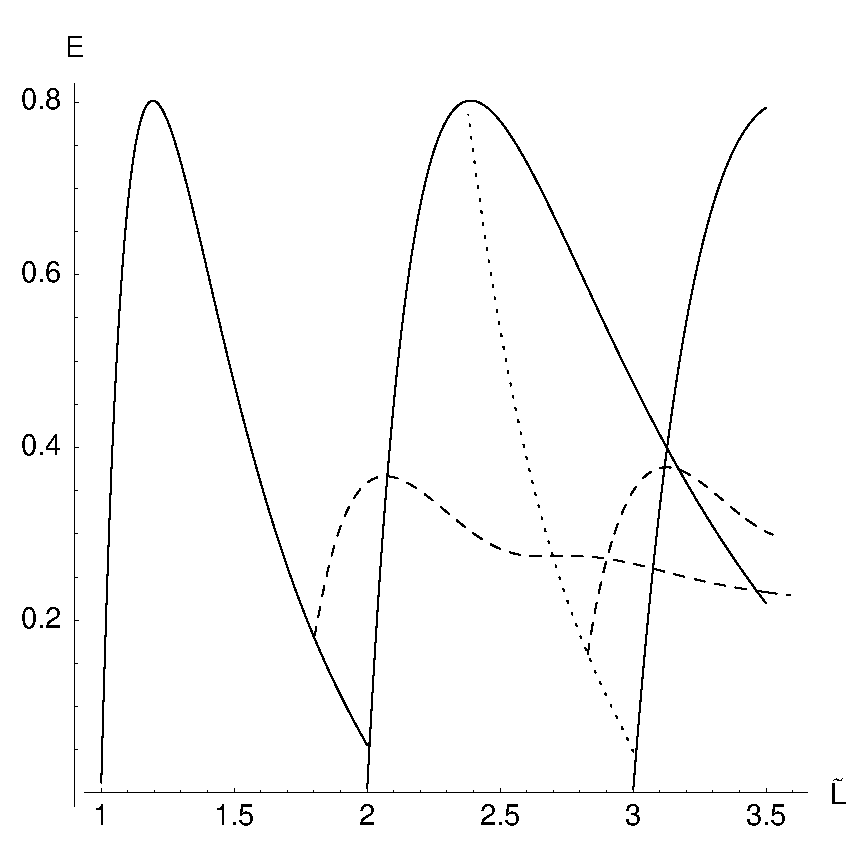
\includegraphics{../../rpo_ks/figs/ksBifDiag.eps}}

\Large

\psframe*[linecolor=white](-6.5,6)(-5.5,7)
\psframe*[linecolor=white](6,-6.5)(7.2,-5.5)

\rput(-7.3,0.5){$E$} \rput(0,-7){$\tilde{L}$}

\psline[linewidth=1pt]{->}(3.4,-5.5)(4.0,-6.0)\rput(3.1,-5.5){E$_0$}
\psline[linewidth=1pt]{->}(3.4,-4.5)(4.0,-4.2)\rput(3.1,-4.5){E$_1$}
\psline[linewidth=1pt]{->}(3.4,-3.4)(4.0,-3.0)\rput(3.1,-3.5){E$_2$}
\psline[linewidth=1pt]{->}(3.4,5.25)(4.0,5.25)\rput(3.1,5.2){E$_3$}
\psline[linewidth=1pt]{->}(4.7,-2.5)(4.05,-2.7)\rput(5.5,-2.5){TW$_{\pm1}$}
\psline[linewidth=1pt]{->}(4.7,-1.0)(4.05,-1.7)\rput(5.5,-1.0){TW$_{\pm2}$}

% Use grid command below to place objects at specified coordinates.
%\psgrid[subgriddiv=1,griddots=10](-8,-8)(7,7)
}
\end{document}
